\subsubsection{Descrizione}
In questo modulo, chiamato \textbf{Back-end\ped{G}}, viene gestita la logica interna del sito \nameproject. In particolare viene amministrato l'accesso al lato \textbf{business} dell'applicativo, e la parte relativa alla persistenza dei dati salvati all'interno dei servizi offerti da Amazon AWS\ped{G}. L'architettura generale del modulo è basata sui microservizi offerti dalle chiamate API, i quali hanno una base in comune sviluppata a \textbf{layer}, dove i tre layer principali sono:
\begin{itemize}
	\item \textbf{Handler\ped{G} delle API\ped{G}}: gestori delle richieste suddivise per dominio;
	\item \textbf{Model}: gestione logica dei modelli delle entità rappresentate (prodotto, utente...);
	\item \textbf{Services}: gestione dei servizi Amazon AWS\ped{G} e complementari.
\end{itemize} Il modulo \textbf{Front-end\ped{G}} interagisce con il modulo \textbf{Back-end\ped{G}} attraverso delle chiamate API\ped{G} esposte del servizio Amazon API Gateway. Tali API\ped{G} sono divise per dominio relativo all'oggetto con cui si vuole interagire e alla sua funzionalità (es. inserimento di un nuovo prodotto). L'handler\ped{G} gestisce la richiesta in base alla propria funzionalità e smista la relativa richiesta, dopo un opportuno controllo, sul \textbf{layer dei servizi} (dove necessario). I servizi offerti comprendono l'interfacciamento con DynamoDB, Stripe, S3, Nodemailer, Cognito. Inoltre, sempre dove necessario, l'handler\ped{G} della richiesta può interfacciarsi con il \textbf{layer dei modelli} degli oggetti (prodotto, utente ecc..) i quali forniranno supporto per la gestione logica di tali elementi.

\vspace{1cm}

\begin{figure}[H]
\centering
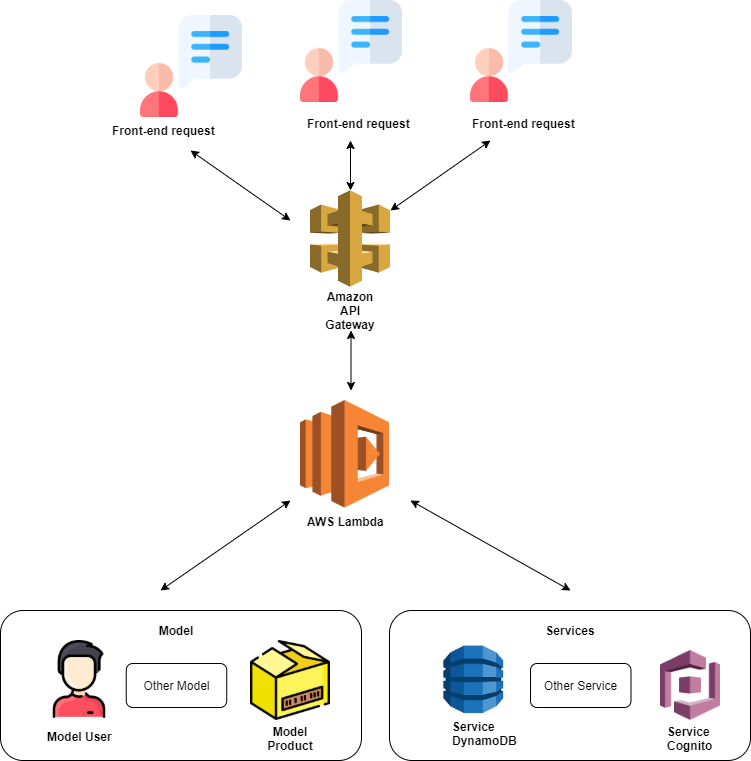
\includegraphics[scale=0.40]{res/Architettura/Backend/img/layerBack-end.png}\\
\caption{Layer del modulo Back-end\ped{G}}
\end{figure}